% Created by tikzDevice version 0.12 on 2019-03-30 20:59:36
% !TEX encoding = UTF-8 Unicode
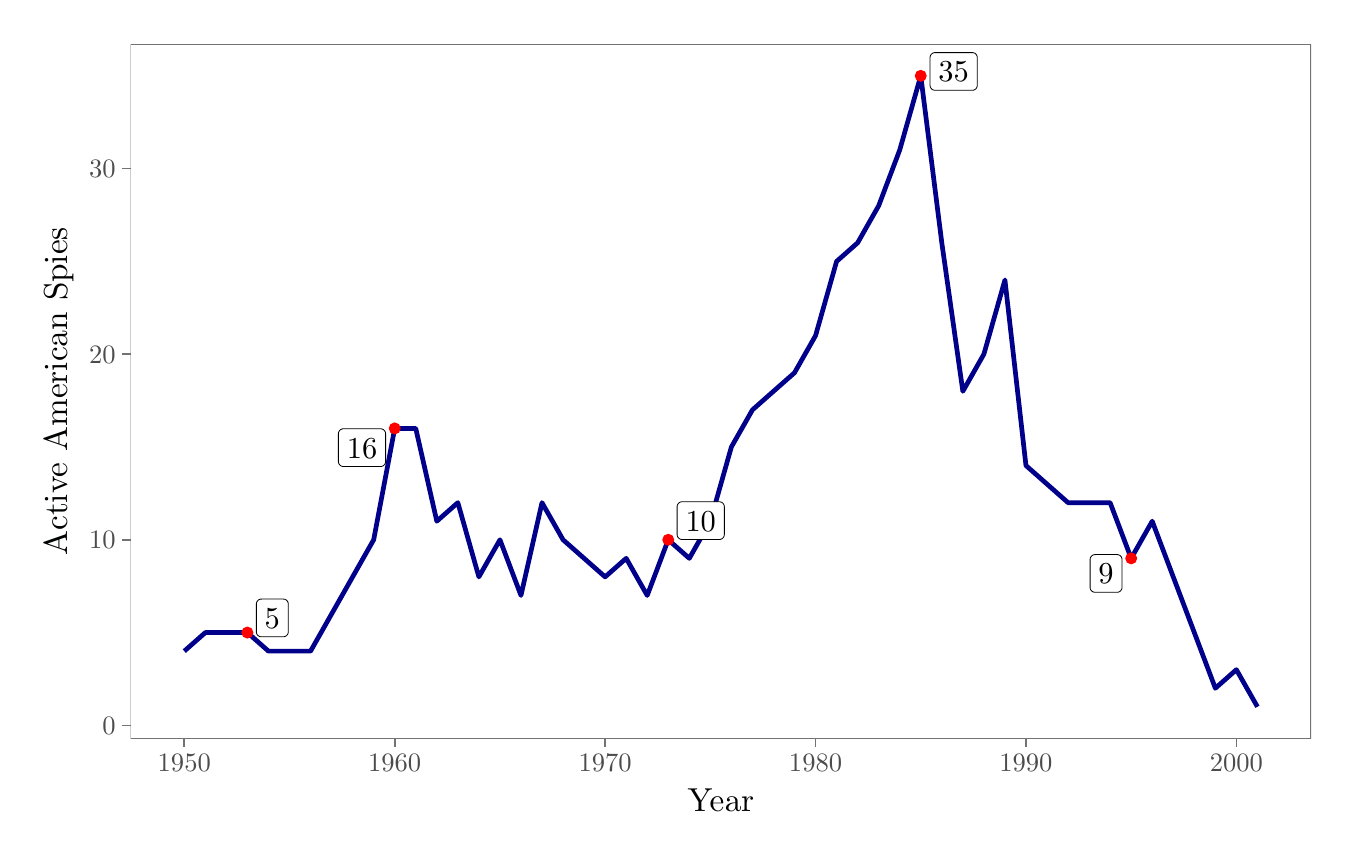
\begin{tikzpicture}[x=1pt,y=1pt]
\definecolor{fillColor}{RGB}{255,255,255}
\path[use as bounding box,fill=fillColor,fill opacity=0.00] (0,0) rectangle (469.75,289.08);
\begin{scope}
\path[clip] (  0.00,  0.00) rectangle (469.75,289.08);
\definecolor{drawColor}{RGB}{255,255,255}
\definecolor{fillColor}{RGB}{255,255,255}

\path[draw=drawColor,line width= 0.6pt,line join=round,line cap=round,fill=fillColor] (  0.00,  0.00) rectangle (469.76,289.08);
\end{scope}
\begin{scope}
\path[clip] ( 37.21, 32.28) rectangle (463.75,283.08);
\definecolor{fillColor}{RGB}{255,255,255}

\path[fill=fillColor] ( 37.21, 32.28) rectangle (463.75,283.08);
\definecolor{drawColor}{RGB}{0,0,139}

\path[draw=drawColor,line width= 1.7pt,line join=round] ( 56.59, 63.79) --
	( 64.20, 70.50) --
	( 71.80, 70.50) --
	( 79.40, 70.50) --
	( 87.01, 63.79) --
	( 94.61, 63.79) --
	(102.22, 63.79) --
	(109.82, 77.21) --
	(117.42, 90.62) --
	(125.03,104.03) --
	(132.63,144.27) --
	(140.23,144.27) --
	(147.84,110.74) --
	(155.44,117.44) --
	(163.04, 90.62) --
	(170.65,104.03) --
	(178.25, 83.91) --
	(185.85,117.44) --
	(193.46,104.03) --
	(201.06, 97.32) --
	(208.66, 90.62) --
	(216.27, 97.32) --
	(223.87, 83.91) --
	(231.47,104.03) --
	(239.08, 97.32) --
	(246.68,110.74) --
	(254.28,137.56) --
	(261.89,150.97) --
	(269.49,157.68) --
	(277.09,164.38) --
	(284.70,177.80) --
	(292.30,204.62) --
	(299.90,211.33) --
	(307.51,224.74) --
	(315.11,244.86) --
	(322.71,271.68) --
	(330.32,211.33) --
	(337.92,157.68) --
	(345.52,171.09) --
	(353.13,197.91) --
	(360.73,130.85) --
	(368.33,124.15) --
	(375.94,117.44) --
	(383.54,117.44) --
	(391.14,117.44) --
	(398.75, 97.32) --
	(406.35,110.74) --
	(413.95, 90.62) --
	(421.56, 70.50) --
	(429.16, 50.38) --
	(436.76, 57.09) --
	(444.37, 43.68);
\definecolor{drawColor}{RGB}{255,0,0}
\definecolor{fillColor}{RGB}{255,0,0}

\path[draw=drawColor,line width= 0.4pt,line join=round,line cap=round,fill=fillColor] ( 79.40, 70.50) circle (  1.96);

\path[draw=drawColor,line width= 0.4pt,line join=round,line cap=round,fill=fillColor] (132.63,144.27) circle (  1.96);

\path[draw=drawColor,line width= 0.4pt,line join=round,line cap=round,fill=fillColor] (231.47,104.03) circle (  1.96);

\path[draw=drawColor,line width= 0.4pt,line join=round,line cap=round,fill=fillColor] (322.71,271.68) circle (  1.96);

\path[draw=drawColor,line width= 0.4pt,line join=round,line cap=round,fill=fillColor] (398.75, 97.32) circle (  1.96);
\end{scope}
\begin{scope}
\path[clip] ( 37.21, 32.28) rectangle (463.75,283.08);
\definecolor{drawColor}{RGB}{0,0,0}
\definecolor{fillColor}{RGB}{255,255,255}

\path[draw=drawColor,line width= 0.3pt,line join=round,line cap=round,fill=fillColor] ( 84.43, 68.98) --
	( 92.36, 68.98) --
	( 92.29, 68.98) --
	( 92.58, 68.99) --
	( 92.86, 69.05) --
	( 93.14, 69.15) --
	( 93.39, 69.30) --
	( 93.61, 69.48) --
	( 93.81, 69.70) --
	( 93.96, 69.94) --
	( 94.08, 70.21) --
	( 94.15, 70.49) --
	( 94.17, 70.78) --
	( 94.17, 70.78) --
	( 94.17, 80.80) --
	( 94.17, 80.80) --
	( 94.15, 81.09) --
	( 94.08, 81.37) --
	( 93.96, 81.64) --
	( 93.81, 81.88) --
	( 93.61, 82.10) --
	( 93.39, 82.28) --
	( 93.14, 82.43) --
	( 92.86, 82.53) --
	( 92.58, 82.59) --
	( 92.36, 82.60) --
	( 84.43, 82.60) --
	( 84.65, 82.59) --
	( 84.36, 82.60) --
	( 84.07, 82.57) --
	( 83.79, 82.49) --
	( 83.53, 82.36) --
	( 83.29, 82.20) --
	( 83.08, 81.99) --
	( 82.91, 81.76) --
	( 82.77, 81.50) --
	( 82.68, 81.23) --
	( 82.63, 80.94) --
	( 82.63, 80.80) --
	( 82.63, 70.78) --
	( 82.63, 70.93) --
	( 82.63, 70.64) --
	( 82.68, 70.35) --
	( 82.77, 70.08) --
	( 82.91, 69.82) --
	( 83.08, 69.59) --
	( 83.29, 69.38) --
	( 83.53, 69.22) --
	( 83.79, 69.09) --
	( 84.07, 69.01) --
	( 84.36, 68.98) --
	cycle;
\end{scope}
\begin{scope}
\path[clip] ( 37.21, 32.28) rectangle (463.75,283.08);
\definecolor{drawColor}{RGB}{0,0,0}

\node[text=drawColor,anchor=base,inner sep=0pt, outer sep=0pt, scale=  1.10] at ( 88.40, 71.99) {5};
\end{scope}
\begin{scope}
\path[clip] ( 37.21, 32.28) rectangle (463.75,283.08);
\definecolor{drawColor}{RGB}{0,0,0}
\definecolor{fillColor}{RGB}{255,255,255}

\path[draw=drawColor,line width= 0.3pt,line join=round,line cap=round,fill=fillColor] (114.09,130.51) --
	(127.53,130.51) --
	(127.46,130.51) --
	(127.75,130.52) --
	(128.03,130.58) --
	(128.31,130.68) --
	(128.56,130.83) --
	(128.78,131.01) --
	(128.98,131.23) --
	(129.13,131.47) --
	(129.25,131.74) --
	(129.32,132.02) --
	(129.34,132.31) --
	(129.34,132.31) --
	(129.34,142.33) --
	(129.34,142.33) --
	(129.32,142.62) --
	(129.25,142.90) --
	(129.13,143.17) --
	(128.98,143.41) --
	(128.78,143.63) --
	(128.56,143.81) --
	(128.31,143.96) --
	(128.03,144.06) --
	(127.75,144.12) --
	(127.53,144.13) --
	(114.09,144.13) --
	(114.30,144.12) --
	(114.01,144.13) --
	(113.72,144.10) --
	(113.45,144.02) --
	(113.18,143.89) --
	(112.94,143.73) --
	(112.73,143.52) --
	(112.56,143.29) --
	(112.42,143.03) --
	(112.33,142.76) --
	(112.28,142.47) --
	(112.28,142.33) --
	(112.28,132.31) --
	(112.28,132.46) --
	(112.28,132.17) --
	(112.33,131.88) --
	(112.42,131.61) --
	(112.56,131.35) --
	(112.73,131.12) --
	(112.94,130.91) --
	(113.18,130.75) --
	(113.45,130.62) --
	(113.72,130.54) --
	(114.01,130.51) --
	cycle;
\end{scope}
\begin{scope}
\path[clip] ( 37.21, 32.28) rectangle (463.75,283.08);
\definecolor{drawColor}{RGB}{0,0,0}

\node[text=drawColor,anchor=base,inner sep=0pt, outer sep=0pt, scale=  1.10] at (120.81,133.52) {16};
\end{scope}
\begin{scope}
\path[clip] ( 37.21, 32.28) rectangle (463.75,283.08);
\definecolor{drawColor}{RGB}{0,0,0}
\definecolor{fillColor}{RGB}{255,255,255}

\path[draw=drawColor,line width= 0.3pt,line join=round,line cap=round,fill=fillColor] (236.48,104.14) --
	(249.93,104.14) --
	(249.86,104.14) --
	(250.15,104.15) --
	(250.43,104.21) --
	(250.70,104.31) --
	(250.96,104.46) --
	(251.18,104.64) --
	(251.37,104.86) --
	(251.53,105.11) --
	(251.64,105.37) --
	(251.71,105.66) --
	(251.74,105.95) --
	(251.74,105.95) --
	(251.74,115.96) --
	(251.74,115.96) --
	(251.71,116.25) --
	(251.64,116.53) --
	(251.53,116.80) --
	(251.37,117.04) --
	(251.18,117.26) --
	(250.96,117.45) --
	(250.70,117.59) --
	(250.43,117.69) --
	(250.15,117.75) --
	(249.93,117.77) --
	(236.48,117.77) --
	(236.70,117.75) --
	(236.41,117.76) --
	(236.12,117.73) --
	(235.84,117.65) --
	(235.58,117.52) --
	(235.34,117.36) --
	(235.13,117.16) --
	(234.96,116.92) --
	(234.82,116.67) --
	(234.73,116.39) --
	(234.68,116.10) --
	(234.68,115.96) --
	(234.68,105.95) --
	(234.68,106.09) --
	(234.68,105.80) --
	(234.73,105.51) --
	(234.82,105.24) --
	(234.96,104.98) --
	(235.13,104.75) --
	(235.34,104.55) --
	(235.58,104.38) --
	(235.84,104.26) --
	(236.12,104.18) --
	(236.41,104.14) --
	cycle;
\end{scope}
\begin{scope}
\path[clip] ( 37.21, 32.28) rectangle (463.75,283.08);
\definecolor{drawColor}{RGB}{0,0,0}

\node[text=drawColor,anchor=base,inner sep=0pt, outer sep=0pt, scale=  1.10] at (243.21,107.15) {10};
\end{scope}
\begin{scope}
\path[clip] ( 37.21, 32.28) rectangle (463.75,283.08);
\definecolor{drawColor}{RGB}{0,0,0}
\definecolor{fillColor}{RGB}{255,255,255}

\path[draw=drawColor,line width= 0.3pt,line join=round,line cap=round,fill=fillColor] (327.88,266.44) --
	(341.33,266.44) --
	(341.26,266.44) --
	(341.55,266.45) --
	(341.83,266.51) --
	(342.11,266.62) --
	(342.36,266.76) --
	(342.58,266.94) --
	(342.78,267.16) --
	(342.93,267.41) --
	(343.04,267.68) --
	(343.11,267.96) --
	(343.14,268.25) --
	(343.14,268.25) --
	(343.14,278.26) --
	(343.14,278.26) --
	(343.11,278.55) --
	(343.04,278.83) --
	(342.93,279.10) --
	(342.78,279.35) --
	(342.58,279.56) --
	(342.36,279.75) --
	(342.11,279.89) --
	(341.83,280.00) --
	(341.55,280.05) --
	(341.33,280.07) --
	(327.88,280.07) --
	(328.10,280.05) --
	(327.81,280.07) --
	(327.52,280.03) --
	(327.24,279.95) --
	(326.98,279.83) --
	(326.74,279.66) --
	(326.53,279.46) --
	(326.36,279.23) --
	(326.22,278.97) --
	(326.13,278.69) --
	(326.08,278.41) --
	(326.08,278.26) --
	(326.08,268.25) --
	(326.08,268.39) --
	(326.08,268.10) --
	(326.13,267.82) --
	(326.22,267.54) --
	(326.36,267.28) --
	(326.53,267.05) --
	(326.74,266.85) --
	(326.98,266.68) --
	(327.24,266.56) --
	(327.52,266.48) --
	(327.81,266.44) --
	cycle;
\end{scope}
\begin{scope}
\path[clip] ( 37.21, 32.28) rectangle (463.75,283.08);
\definecolor{drawColor}{RGB}{0,0,0}

\node[text=drawColor,anchor=base,inner sep=0pt, outer sep=0pt, scale=  1.10] at (334.61,269.45) {35};
\end{scope}
\begin{scope}
\path[clip] ( 37.21, 32.28) rectangle (463.75,283.08);
\definecolor{drawColor}{RGB}{0,0,0}
\definecolor{fillColor}{RGB}{255,255,255}

\path[draw=drawColor,line width= 0.3pt,line join=round,line cap=round,fill=fillColor] (385.71, 85.05) --
	(393.63, 85.05) --
	(393.56, 85.05) --
	(393.85, 85.06) --
	(394.14, 85.12) --
	(394.41, 85.22) --
	(394.66, 85.37) --
	(394.89, 85.55) --
	(395.08, 85.77) --
	(395.23, 86.02) --
	(395.35, 86.28) --
	(395.42, 86.57) --
	(395.44, 86.86) --
	(395.44, 86.86) --
	(395.44, 96.87) --
	(395.44, 96.87) --
	(395.42, 97.16) --
	(395.35, 97.44) --
	(395.23, 97.71) --
	(395.08, 97.95) --
	(394.89, 98.17) --
	(394.66, 98.36) --
	(394.41, 98.50) --
	(394.14, 98.60) --
	(393.85, 98.66) --
	(393.63, 98.68) --
	(385.71, 98.68) --
	(385.92, 98.66) --
	(385.63, 98.67) --
	(385.35, 98.64) --
	(385.07, 98.56) --
	(384.80, 98.43) --
	(384.56, 98.27) --
	(384.35, 98.07) --
	(384.18, 97.83) --
	(384.04, 97.58) --
	(383.95, 97.30) --
	(383.91, 97.01) --
	(383.90, 96.87) --
	(383.90, 86.86) --
	(383.91, 87.00) --
	(383.91, 86.71) --
	(383.95, 86.42) --
	(384.04, 86.15) --
	(384.18, 85.89) --
	(384.35, 85.66) --
	(384.56, 85.46) --
	(384.80, 85.29) --
	(385.07, 85.17) --
	(385.35, 85.09) --
	(385.63, 85.05) --
	cycle;
\end{scope}
\begin{scope}
\path[clip] ( 37.21, 32.28) rectangle (463.75,283.08);
\definecolor{drawColor}{RGB}{0,0,0}

\node[text=drawColor,anchor=base,inner sep=0pt, outer sep=0pt, scale=  1.10] at (389.67, 88.06) {9};
\definecolor{drawColor}{gray}{0.45}

\path[draw=drawColor,line width= 0.6pt,line join=round,line cap=round] ( 37.21, 32.28) rectangle (463.75,283.08);
\end{scope}
\begin{scope}
\path[clip] (  0.00,  0.00) rectangle (469.75,289.08);
\definecolor{drawColor}{gray}{0.30}

\node[text=drawColor,anchor=base east,inner sep=0pt, outer sep=0pt, scale=  0.96] at ( 31.81, 33.66) {0};

\node[text=drawColor,anchor=base east,inner sep=0pt, outer sep=0pt, scale=  0.96] at ( 31.81,100.72) {10};

\node[text=drawColor,anchor=base east,inner sep=0pt, outer sep=0pt, scale=  0.96] at ( 31.81,167.78) {20};

\node[text=drawColor,anchor=base east,inner sep=0pt, outer sep=0pt, scale=  0.96] at ( 31.81,234.84) {30};
\end{scope}
\begin{scope}
\path[clip] (  0.00,  0.00) rectangle (469.75,289.08);
\definecolor{drawColor}{gray}{0.45}

\path[draw=drawColor,line width= 0.6pt,line join=round] ( 34.21, 36.97) --
	( 37.21, 36.97);

\path[draw=drawColor,line width= 0.6pt,line join=round] ( 34.21,104.03) --
	( 37.21,104.03);

\path[draw=drawColor,line width= 0.6pt,line join=round] ( 34.21,171.09) --
	( 37.21,171.09);

\path[draw=drawColor,line width= 0.6pt,line join=round] ( 34.21,238.15) --
	( 37.21,238.15);
\end{scope}
\begin{scope}
\path[clip] (  0.00,  0.00) rectangle (469.75,289.08);
\definecolor{drawColor}{gray}{0.45}

\path[draw=drawColor,line width= 0.6pt,line join=round] ( 56.59, 29.28) --
	( 56.59, 32.28);

\path[draw=drawColor,line width= 0.6pt,line join=round] (132.63, 29.28) --
	(132.63, 32.28);

\path[draw=drawColor,line width= 0.6pt,line join=round] (208.66, 29.28) --
	(208.66, 32.28);

\path[draw=drawColor,line width= 0.6pt,line join=round] (284.70, 29.28) --
	(284.70, 32.28);

\path[draw=drawColor,line width= 0.6pt,line join=round] (360.73, 29.28) --
	(360.73, 32.28);

\path[draw=drawColor,line width= 0.6pt,line join=round] (436.76, 29.28) --
	(436.76, 32.28);
\end{scope}
\begin{scope}
\path[clip] (  0.00,  0.00) rectangle (469.75,289.08);
\definecolor{drawColor}{gray}{0.30}

\node[text=drawColor,anchor=base,inner sep=0pt, outer sep=0pt, scale=  0.96] at ( 56.59, 20.26) {1950};

\node[text=drawColor,anchor=base,inner sep=0pt, outer sep=0pt, scale=  0.96] at (132.63, 20.26) {1960};

\node[text=drawColor,anchor=base,inner sep=0pt, outer sep=0pt, scale=  0.96] at (208.66, 20.26) {1970};

\node[text=drawColor,anchor=base,inner sep=0pt, outer sep=0pt, scale=  0.96] at (284.70, 20.26) {1980};

\node[text=drawColor,anchor=base,inner sep=0pt, outer sep=0pt, scale=  0.96] at (360.73, 20.26) {1990};

\node[text=drawColor,anchor=base,inner sep=0pt, outer sep=0pt, scale=  0.96] at (436.76, 20.26) {2000};
\end{scope}
\begin{scope}
\path[clip] (  0.00,  0.00) rectangle (469.75,289.08);
\definecolor{drawColor}{RGB}{1,2,2}

\node[text=drawColor,anchor=base,inner sep=0pt, outer sep=0pt, scale=  1.20] at (250.48,  6.00) {Year};
\end{scope}
\begin{scope}
\path[clip] (  0.00,  0.00) rectangle (469.75,289.08);
\definecolor{drawColor}{RGB}{1,2,2}

\node[text=drawColor,rotate= 90.00,anchor=base,inner sep=0pt, outer sep=0pt, scale=  1.20] at ( 14.26,157.68) {Active American Spies};
\end{scope}
\end{tikzpicture}
